\section{Волновые процессы в сложных биологических средах}

Численное изучение физиологических и патологических процессов, происходящих в организме человека, позволяет получить новые качественные и количественные характеристики функционирования органов в различных условиях и протекающих в них нормальных и патологических процессов, что необходимо для прогнозирования их развития, предсказания последствий патологий, выдачи медицинских рекомендаций и разработки новых принципов диагностики на ранних стадиях различных заболеваний.

На сегодняшний день медицина является экспериментальной наукой, ориентированной на констатацию фактов и выдачу рекомендаций в части операционных или медикаментозных средств для ослабления патологических процессов. Проблема построения математических моделей функционирования различных органов остается практически открытой.

Наиболее сложной проблемой при построении моделей органов и процессов в них является экспериментальная верификация расчетных данных, так как соответствующие эксперименты практически отсутствуют. Более того, некоторые процессы в данной области изучать экспериментально крайне затруднительно, если вообще возможно. По этой причине и появились предложения со стороны медицинских специалистов изучать подобные процессы методами численного моделирования.

Математическое моделирование, как метод исследования в данном случае обладает рядом очевидных достоинств: небольшая стоимость численного эксперимента, доступная широта диапазона изменения основных параметров, полнота получаемой в результате картины динамики скоростей, напряжений и деформаций во всем объеме рассматриваемой системы.

\clearpage
\newpage

\subsection{Задача о черепно-мозговой травме}

В данном разделе рассматривается задача о численном моделировании сеточно-характеристическим методом механических процессов, протекающих в системе череп-мозг при различных динамических воздействиях. Эта задача является актуальной с точки зрения выяснения механизмов повреждаемости тканей мозга при различных типах внешней нагрузки.

Объяснение явлениям, наблюдаемым при черепно-мозговой травме (далее по тексту — ЧМТ) может дать только изучение сложных процессов, протекающих в неоднородной биологической конструкции, которую представляет из себя голова человека (рис. \ref{pic:cranium_scheme}). Слоистая конструкция покровов головного мозга ослабляет действие продольных упругих волн (за счёт пористого слоя черепной коробки), поперечных упругих волн (за счёт слоя ликвора под костной частью), напряжений, вызванных нормальными, а также скользящими ударами. Можно предположить, что именно сложная волновая картина, обусловленная как геометрическими особенностями анатомии черепа, так и различием механических свойств компонентов системы череп-мозг, определяет пространственное распределение областей напряжений.

\begin{figure}[htp]
\centering
\begin{subfigure}[b]{0.6\textwidth}
\centering
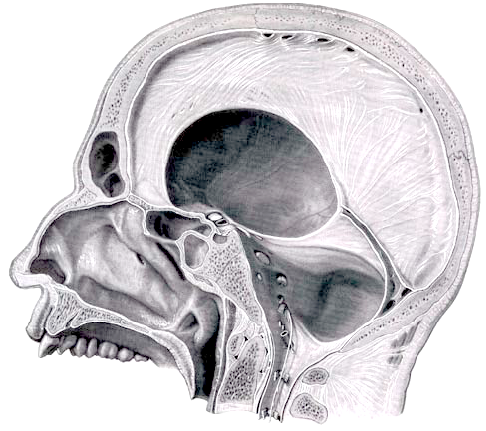
\includegraphics[width=\textwidth]{png/cranium/real-scheme-01.png}
\end{subfigure}
\begin{subfigure}[b]{0.6\textwidth}
\centering
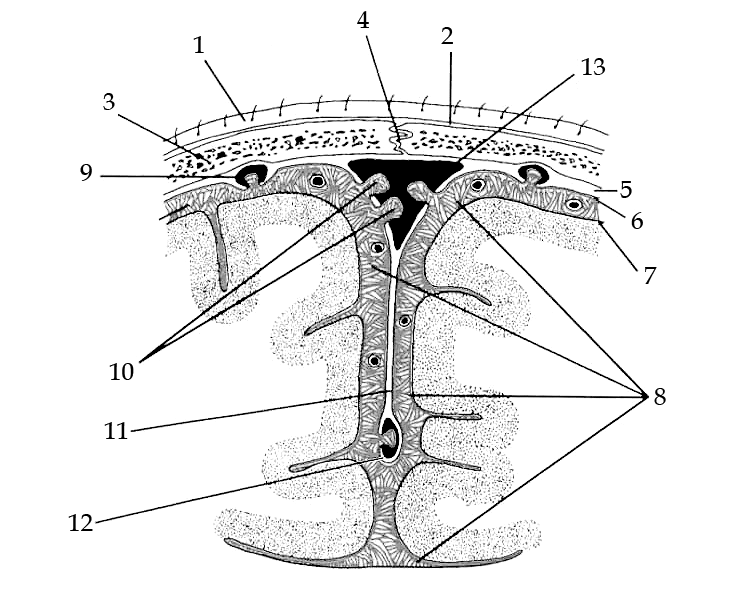
\includegraphics[width=\textwidth]{png/cranium/real-scheme-02.png}
\end{subfigure}
\caption{a – кости и твердая оболочка, сагиттальное сечение; б – оболочки мозга (фронтальный срез): 1 – кожа, 2 – надкостница, 3 – кость черепа, 4 – продольный шов, 5 – твердая оболочка, 6 – паутинная оболочка, 7 – сосудистая оболочка, 8 – субарахноидальное пространство, 9 – венозная впадина, 10 – арахноидальные грануляции, 11 – серп большого мозга, 12 – нижний сагиттальный синус (расстояния между оболочками преувеличены)}
\label{pic:cranium_scheme}
\end{figure}

Из нейрохирургической практики известно, что области поражения мозга при черепно-мозговой травме не всегда совпадают с областями, прилежащими к месту удара. Примером этому является известный феномен «противоудара» – при ударе затылком область поражения мозга локализуется в лобной части головы человека.

На сегодняшний день не существует теории, которая предложила бы механизм повреждения мозга при ЧМТ и давала бы исчерпывающее объяснение всем фактам из клинической практики. Наиболее распространенными и успешными являются две теории — механическая и кавитационная.

Механическая теория объясняет возникновение зон поражения в области «противоудара» кинематикой костных пластинок. Согласно этой теории в момент удара пластинчатая кость в области крыши орбиты, больших и малых крыльев основной кости испытывает значительные деформации (до 1 см). Совершая возвратное движение, костная пластина вызывает поражение мозгового вещества. Однако ряд фактов не согласуется с этой теорией. Во-первых, у ряда больных при КТ-исследованиях в первые часы после травмы очагов ушибов мозга не обнаруживается, они возникают позже. Кроме того, такие очаги располагаются не только на поверхностях мозга, непосредственно прилегающих к костным пластинам, но и на полюсных и конвекситальных поверхностях, где с мозгом граничит не пластинчатая, а губчатая кость, которая при травме таких колебательных движений не совершает и мозг повредить не может.

Кавитационная теория строится на предположении, что вследствие ротационного движения мозга или смещения по инерции его массы на противоположной стороне образуется вакуум. Отрицательное давление, действующее в течение нескольких милисекунд, вызывает в текущей жидкости (крови) появление пузырьков газа (кавитацию). Перемещаясь с потоком крови в область более высокого давления, кавитационный пузырек «схлопывается», вызывая при этом гидродинамическую ударную волну, которая и разрушает стенки сосуда. Кавитационная теория хорошо объясняет развитие во времени очагов поражения и отсутствие в начальные моменты времени в них крови и травматически поврежденных клеток. Однако неясно, насколько кавитационные эффекты действительно имеют место в крови сосудов мозга. За пределами теории также тот факт, что локализация повреждений происходит в основном в лобной и височной долях.

По результатам анализа работ, опубликованных в печатных и электронных изданиях, можно сделать вывод о том, что подавляющее количество исследовательских работ в области моделирования ЧМТ было проведено за рубежом c применением различных вариаций методов конечных элементов (МКЭ) (в частности, \cite{zhou}, \cite{kuijpers}, \cite{chu}, \cite{claessens}). Подробный обзор зарубежных работ, посвященных численному исследованию ЧМТ, выполнен в \cite{agapov_diser}.

Несмотря на то, что моделирование головного отдела человека с помощью МКЭ в последние десять лет интенсивно развивается, оно еще далеко от того, чтобы иметь возможность объяснить механизмы повреждения мозга и предсказать последствия ЧМТ. Такие вопросы, как реология биоматериалов, составляющих голову человека, механическое взаимодействие поверхностей мозга и черепа, воздействие желудочков и пустот на распределение напряжений, рассмотрение многослойного строения оболочек мозга с воспроизведением его точной геометрии требуют дальнейшего исследования. 

В работе \cite{zhou} был предложен ряд двумерных моделей для трансверсального и сагиттального сечений для анализа влияния различий в механических свойствах белого и серого вещества на распределение максимальных сдвиговых напряжений. Автор показал, что различие в механических свойствах серого и белого веществ, а также включение в модель желудочков необходимо для соответствия вычисленного распределения максимальных сдвиговых напряжений наблюдаемым аксональным повреждениям в белом веществе. В данной модели желудочки описывались жидкостными элементами, а модуль Юнга белого вещества был на 60\% больше, чем серого. 

В исследовании \cite{kuijpers} использовалась двумерная модель вертикального сечения головы человека. Контакт череп-мозг моделировался двумя способами -- жесткое сцепление и скольжение с возможностью отрыва. Кроме того, большое отверстие также моделировалось тремя способами -- жесткое сцепление, скольжение с возможностью отрыва, незакрепленное. Сравнение с экспериментом показало наилучшее соответствие величины давления в месте удара в случае скользящего контакта, в то время как модели с жестким сцеплением показали результат, наиболее далекий от действительности. Ни одна из моделей не показала соответствия давлений в месте противоудара, что может объясняться неспособностью контактного алгоритма противостоять растягивающим нагрузкам. Авторы заключили, что величины давления как в месте удара, так и в месте противоудара намного более чувствительны к способу моделирования контакта череп-мозг, чем к наличию или отсутствию свободного большого отверстия. 

Смещение мозга относительно черепа описаны более пятидесяти лет назад. Это вызывало особый интерес к численному моделированию этого явления. Моделирование внутричерепной жидкости линейно-упругими элементами с малым сдвиговым модулем \cite{zhou} показало, что этот подход вносит дополнительные касательные напряжения между черепом и мозгом, а также снижают устойчивость вычислений вследствие вырождения элементов. Другим подходом является введение контактных условий на границе череп-мозг. Конкретные условия различаются у разных авторов, от жесткого сцепления до скольжения с трением. Было проведено некоторое количество сравнительных исследований с использованием различных контактных условий \cite{claessens}. Все они приводят к заключению, что эффект ударного воздействия на голову человека чувствителен к способу моделирования взаимодействия череп-мозг. 

Основные трудности, возникающие в большинстве современных МКЭ моделей ударных воздействий на черепно-мозговой отдел человека, возникают в связи с высокой чувствительностью результата к аккуратному моделированию контактных взаимодействий черепа и мозга, а также к учету различных структурных неоднородностей в мозге.

Кроме того, методы конечных элементов изначально предназначены для расчета статических процессов, в то время как в данной задаче существенную роль играют динамические волновые процессы.

Это дает основание полагать, что применение иных классов численных методов может служить эффективным средством повышения точности существующих моделей. Одним из таких классов является класс сеточно-характеристических методов, известных более аккуратной формулировкой граничных и контактных условий, а также способностью более адекватно описывать сложные волновые картины распространения возмущений в сильно гетерогенной среде. В то же время наличие сложной геометрии свидетельствует о необходимости обобщения и распространения существующих сеточно-характеристических методов на случай нерегулярных сеток и трех пространственных переменных.

Изучение черепно-мозговой травмы сеточно-характеристическими численными методами было начато в работе \cite{biomech_first}. В данной работе авторы рассматривают общие подходы к численному моделированию различных динамических задач биомеханики, в том числе представлены расчеты распространения возмущений в системе череп-мозг на примере двухкомпонентных двумерных моделей (сагитальная и трансверсальная проекции). Полученные результаты показывают перспективность использования сеточно-характеристических методов – на использованной простейшей модели видны возможности формирования зон удара и противоудара, что согласуется с данными клинической практики.

Дальнейшее развитие применение сеточно-характеристических численных методов для моделирования ЧМТ получило в работе \cite{agapov_diser}. Эта работа, по-видимому, является наиболее полной на сегодняшний день в данной области. В данной работе сформулирован ряд двумерных математических моделей механической реакции системы череп-мозг на ударное воздействие, позволяющих численно определить распределение в пространстве пиковых механических нагрузок и деформаций тканей мозга. В работе проведен анализ влияния некоторых параметров на результат моделирования.

\begin{itemize}

\item Геометрия компонентов системы. В работе использовались три модели: простейшая двухкомпонентная модель череп-мозг, модель с учетом желудочков большого мозга, модель с учетом желудочков и серпа большого мозга. Получено, что все рассмотренные компоненты оказывают заметное влияние на рассматриваемые биомеханические процессы.

\item Различные варианты контактных условий на границе череп-мозг. Использовались условия полного слипания и свободного скольжения. При использовании условий свободного скольжения получены результаты, гораздо лучше соответствующие данным клинической практики. Этот факт очевидно связан с тем, что в реальной системе между черепом и мозгом расположен слой внутричерепной жидкости. Таким образом, реальное контактное условие - «два твердых тела через тонкий слой жидкости», которое при малых относительных скоростях тел хорошо приближается условием свободного скольжения. Аналогичные результаты получены в работах \cite{kuijpers} и \cite{claessens}.

\item Зависимость максимальных отрицательных и положительных, а также сдвиговых напряжений от направления удара для разных моделей. Получено, что отрицательные и положительные напряжения слабо зависят от использованных геометрических моделей и условий на контактных границах, в то время как для сдвиговых нагрузок зависимость от них значительная.

\end{itemize}

Также в работе \cite{agapov_diser} получено, что зоны повреждений мозга гораздо лучше коррелируют с зонами максимальных сдвигов, чем с зонами сжатий и растяжений. Об этой же особенности говорят и результаты работ \cite{zhou} и \cite{chu}. В свете этого факта особенно интересной становится отмеченная выше зависимость расположения зон максимальных сдвигов от направления удара и от использованной модели.


\clearpage
\newpage

\subsubsection*{Механические процессы в покровах мозга при ударе}

В задаче о черепно-мозговой травме можно выделить несколько характерных особенностей.

\begin{itemize}

\item Большое различие в механических свойствах компонентов биологической системы. Например, модули Юнга костной ткани и мозгового вещества различаются на порядки.

\item Неоднородность внутреннего строения отдельных компонентов. Кости, к примеру, состоят из двух типов ткани -- компактной и губчатой, которые заметно различаются по своим свойствам.

\item Большое количество компонентов системы и их сложная геометрия.

\end{itemize}

Указанные особенности сильно затрудняют моделирование всей системы череп-мозг целиком. Поэтому естественно детально рассмотреть составляющие данной системы по отдельности. Это позволит лучше понять происходящие процессы на микроуровне, а также определить, какие из их свойств и особенностей являются важными для рассматриваемой полной задачи о ЧМТ.

В данной частной задаче исследовались волновые процессы, происходящие в покровах мозга при динамическом нагружении. Рассматривалось прохождение волны нагрузки через череп и ликвор до мозга. 

Данные о строении покровов мозга были взяты из \cite{anatomy_atlas}, соответствующий срез приведен на рис. \ref{pic:cranium_section}.

При моделировании череп был принят состоящим из трех однородных слоев костной ткани – внешнего из компактной, промежуточного из губчатой и внутреннего из компактной, также в модель были включены внутричерепная жидкость (ликвор) и мозговое вещество (рис. \ref{pic:cranium_calc_model}).

Моделировался нормальный удар медленно летящим шариком по черепу. Рассматривалась прямоугольная область, представляющая собой небольшую часть покровов мозга и собственно мозгового вещества (рис. \ref{pic:cranium_calc_model}). На правой границе, соответствующей внешней стенке черепа, ставилось условие свободной границы (нулевые касательные и нормальные напряжения). На трех остальных границах, которые на самом деле свободными не являются, также ставилось условие свободной границы, но при этом геометрия области выбиралась таким образом, чтобы за рассматриваемое время возмущение не успело дойти до этих границ. Расчет различных слоев костной ткани черепа, внутричерепной жидкости и мозгового вещества производился сквозным образом.

\begin{figure}[h]
\center{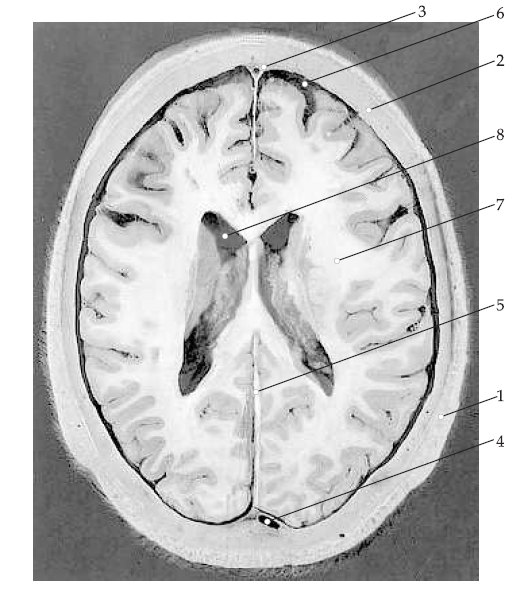
\includegraphics[width=0.6\textwidth]{png/cranium/real-view.png}}
\caption{Трансверсальное сечение головы человека. 1 -- мягкие ткани, 2 -- кости черепа, 3 -- твердая оболочка (dura mater), 4 -- синусы, 5 -- серп большого мозга (falx cerebri), 6 -- ликвор, 7 -- серое и белое мозговое вещество, 8 -- желудочки мозга}
\label{pic:cranium_section}
\end{figure}

\begin{figure}[h]
\center{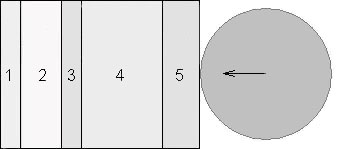
\includegraphics[width=0.6\textwidth]{png/cranium/calc-model.png}}
\caption{Вид расчетной области (размер по вертикали не соблюден). 1 -- мозговое вещество, 2 -- ликвор, 3 -- внутренний слой компактной костной ткани, 4 -- слой губчатой костной ткани, 5 -- внешний слой компактной костной ткани.}
\label{pic:cranium_calc_model}
\end{figure}

Данные обо всех включенных в модель компонентах представлены в таблице \ref{tbl:cranium_elastic_parameters}.

\begin{table}[h]
\centering
\caption{Механические характеристики рассматриваемых биологических материалов}
\begin{tabular}{|c|c|c|c|}
\hline
Компонент & $\rho$, кг/м$^{3}$ & $\lambda$, ГПа & $\mu$, ГПа  \\
\hline
Компактная костная ткань & 1.60 & 7900 & 5270 \\
Губчатая костная ткань & 1.50 & 3975 & 2650 \\
Ликвор & 1.00 & 1700 & 0.001 \\
Мозговое вещество & 1.02 & 1700 & 0.23 \\
\hline
\end{tabular}
\label{tbl:cranium_elastic_parameters}
\end{table}

Коэффициент $\lambda$ для ликвора пересчитан из скорости звука, $\mu$ взят ненулевым, чтобы не создавать вычислительных проблем.

Шарик и череп считались на двух разных сетках. Контактная граница между ними выделялась явным образом, на ней ставились условия свободного скольжения – равенство нормальных напряжений и нормальных компонент скорости и нулевые касательные напряжения.


Влияние различных слоев покровов мозга на распространение волны детально изучалось на одномерной модели. Внешняя нагрузка при этом задавалась в виде прямоугольного импульса длительности 15 мкс. В этом случае амплитуда первичной волны не меняется со временем, что позволяет сделать картину волновых процессов более четкой. На рис. \ref{pic:cranium_1d} представлены графики зависимости напряжения от координаты в различные моменты времени. Ось направлена по внешней нормали, ноль соответствует поверхности черепа. На графиках видно влияние различных слоев покровов мозга на распространение волны и отражение от контактных границ.

\begin{figure}[h]
\centering
\begin{subfigure}[b]{0.6\textwidth}
\centering
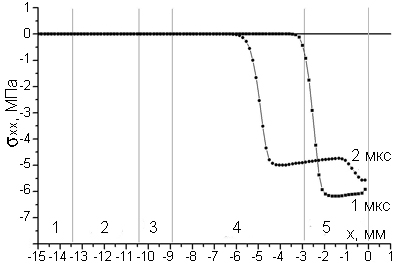
\includegraphics[width=\textwidth]{png/cranium/1d-01.png}
\caption{Отражение от первой контактной границы}
\end{subfigure}
\begin{subfigure}[b]{0.6\textwidth}
\centering
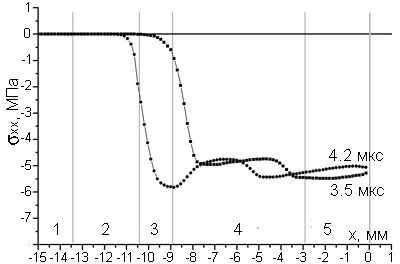
\includegraphics[width=\textwidth]{png/cranium/1d-02.png}
\caption{Прохождение второй контактной границы}
\end{subfigure}
\begin{subfigure}[b]{0.6\textwidth}
\centering
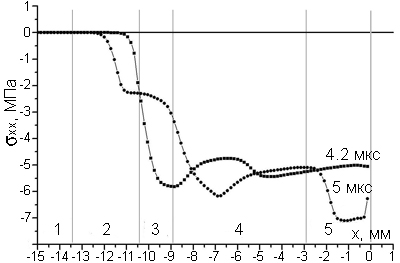
\includegraphics[width=\textwidth]{png/cranium/1d-03.png}
\caption{Прохождение возмущения в ликвор}
\end{subfigure}
\caption{Зависимость напряжения от координаты. 1 -- мозговое вещество, 2 -- ликвор, 3 -- внутренний слой компактной костной ткани, 4 -- слой губчатой костной ткани, 5 -- внешний слой компактной костной ткани.}
\label{pic:cranium_1d}
\end{figure}

Основные расчеты были сделаны на двумерной модели. Моделировался удар шариком из жесткого пластика сантиметрового диаметра, налетающим со скоростью 3 м/с перпендикулярно стенке черепа. Разумеется, такой удар не приводит к травмам. Но принципиальная картина волновых процессов не зависит от скорости шарика, поэтому ее можно выбрать малой для удобства расчетов. На рис. \ref{pic:cranium_2d} изображены изолинии напряжений в различные моменты времени.

\begin{figure}[h]
\centering
\begin{subfigure}[b]{0.15\textwidth}
\centering

\includegraphics[width=\textwidth]{png/cranium/2d-sxx-01.png}
\caption{ }
\end{subfigure}
\begin{subfigure}[b]{0.15\textwidth}
\centering
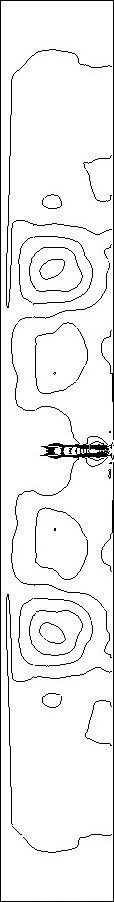
\includegraphics[width=\textwidth]{png/cranium/2d-sxx-02.png}
\caption{ }
\end{subfigure}
\begin{subfigure}[b]{0.15\textwidth}
\centering
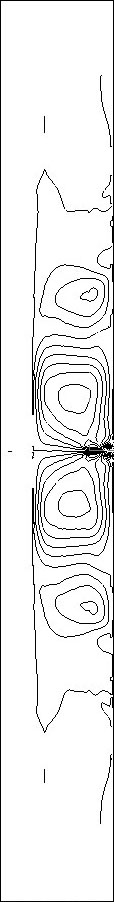
\includegraphics[width=\textwidth]{png/cranium/2d-sxy-01.png}
\caption{ }
\end{subfigure}
\begin{subfigure}[b]{0.15\textwidth}
\centering
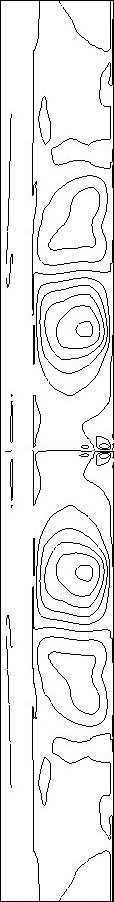
\includegraphics[width=\textwidth]{png/cranium/2d-sxy-02.png}
\caption{ }
\end{subfigure}
\begin{subfigure}[b]{0.15\textwidth}
\centering

\includegraphics[width=\textwidth]{png/cranium/2d-syy-01.png}
\caption{ }
\end{subfigure}
\begin{subfigure}[b]{0.15\textwidth}
\centering
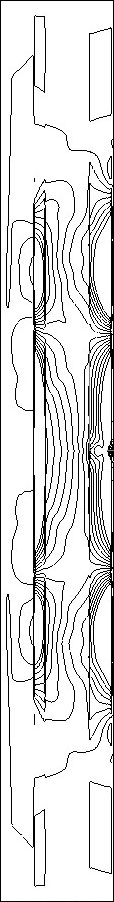
\includegraphics[width=\textwidth]{png/cranium/2d-syy-02.png}
\caption{ }
\end{subfigure}
\caption{Изолинии напряжений. а -- $\sigma_{xx}$ при t = 15 мкс., б -- $\sigma_{xx}$ при t = 25 мкс., в -- $\sigma_{xy}$ при t = 15 мкс., г -- $\sigma_{xy}$ при t = 25 мкс., д -- $\sigma_{yy}$ при t = 15 мкс., е -- $\sigma_{yy}$ при t = 25 мкс. Ось x направлена вправо, ось y -- вверх. Шарик налетает справа.}
\label{pic:cranium_2d}
\end{figure}

На рис. \ref{pic:cranium_2d_1d} представлены одномерные графики зависимости напряжений от координаты. Ось направлена по внешней нормали, ноль соответствует поверхности черепа.

\begin{figure}[h]
\centering
\begin{subfigure}[b]{0.6\textwidth}
\centering
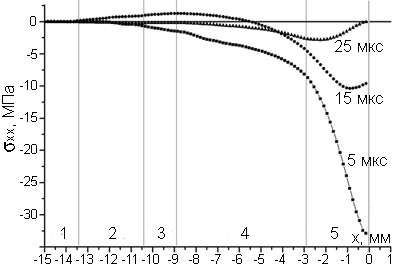
\includegraphics[width=\textwidth]{png/cranium/2d-sxx-1d.png}
\caption{$\sigma_{xx}$}
\end{subfigure}
\begin{subfigure}[b]{0.6\textwidth}
\centering
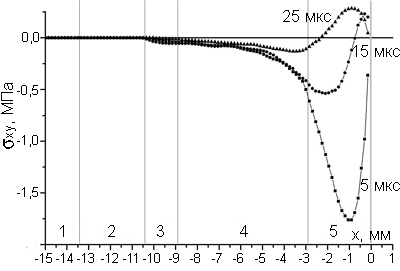
\includegraphics[width=\textwidth]{png/cranium/2d-sxy-1d.png}
\caption{$\sigma_{xy}$}
\end{subfigure}
\begin{subfigure}[b]{0.6\textwidth}
\centering
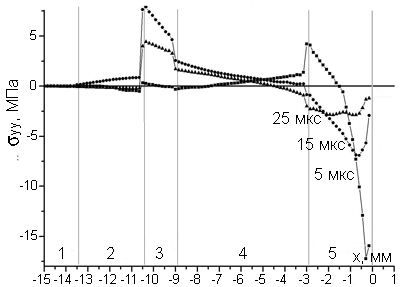
\includegraphics[width=\textwidth]{png/cranium/2d-syy-1d.png}
\caption{$\sigma_{yy}$}
\end{subfigure}
\caption{Зависимость напряжения от координаты. 1 -- мозговое вещество, 2 -- ликвор, 3 -- внутренний слой компактной костной ткани, 4 -- слой губчатой костной ткани, 5 -- внешний слой компактной костной ткани.}
\label{pic:cranium_2d_1d}
\end{figure}

Видно, что покровы мозга уменьшают напряжения во много раз. Сдвиговые напряжения полностью снимаются ликвором, нормальные напряжения ослабляются в стенке черепа на порядки. Отдельно стоит отметить, что нормальные напряжения, действующие вдоль оси y, концентрируются в слоях компактной костной ткани (рис. \ref{pic:cranium_2d_1d}в).

Эффективности покровов мозга как защитной конструкции также способствует то, что коэффициенты Ламе для мозгового вещества на порядки меньше, чем для остальных компонентов системы, при лишь небольших различиях плотности. Это приводит к тому, что возмущения в черепе и ликворе распространяются намного быстрее, чем в мозге. В результате диссипация возмущений в покровах мозга происходит гораздо быстрее, чем их проникновение в мозг. На рис. \ref{pic:cranium_2d} видно, что за время от 15 мкс до 25 мкс после удара возмущения практически не заходят вглубь мозга, а по ликвору и черепу они за это же распространяются на довольно большие расстояния.

Также был выполнен количественный анализ результатов расчетов. В одномерном случае получено, что череп и ликвор снижают нагрузки на мозг в 20-30 раз по сравнению с нагрузками в месте нанесения удара. В двумерном случае нагрузки снижались в 300-400 раз, что связано с отмеченной выше большой скоростью диссипации возмущений. В трехмерном случае следует ожидать еще большего снижения нагрузок. 

\clearpage
\newpage

\subsubsection*{Упрощенная модель покровов мозга}

Картина распространения возмущений в стенке черепа носит явно выраженный волновой характер, наблюдается многократное отражение волн от контактных границ между отдельными компонентами. Соответственно, внутреннее строение рассматриваемой системы может оказывать сильное влияние на происходящие процессы. Таким образом, кажется логичным при дальнейшем моделировании использовать введенную многокомпонентную модель покровов мозга. Но этот подход наталкивается на две сложности.

\begin{itemize}

\item Введенная многокомпонентная модель требует сильного измельчения расчетной сетки, что ведет к уменьшению шага интегрирования.

\item Механические параметры отдельных компонент системы известны неточно. При этом неясно, насколько сильно их изменение скажется на итоговой картине.

\end{itemize}

Поэтому перед применением многокомпонентной модели разумно рассмотреть, насколько ее введение влияет на различные стадии процесса, и понять, когда ее использование разумно, а когда будет слабо сказываться на итоговых результатах.

В многокомпонентной модели череп был принят состоящим из трех однородных слоев костной ткани, также в модель были включены внутричерепная жидкость (ликвор) и мозговое вещество (рис. \ref{pic:cranium_calc_model}). Для сравнения использовались две упрощенные модели. В первой из них слои 3, 4, 5 (рис. \ref{pic:cranium_calc_model}) были объединены в один слой, состоящий их компактной костной ткани. Во второй модели слои объединялись так же, но итоговый слой состоял из губчатой ткани. Таким образом три модели (многокомпонентная и две упрощенные) позволили рассмотреть влияние как сложности модели (числа слоев), так и механических характеристик материала черепа.

Для подробного рассмотрения распространения волн и их взаимодействия с контактными границами была выполнена серия одномерных расчетов.Внешняя нагрузка в одномерном случае задавалась в виде бесконечного прямоугольного импульса 10 МПа.

На рис. \ref{pic:cranium_model1_1d} и \ref{pic:cranium_model2_1d} представлены графики зависимости напряжения от координаты в различные моменты времени для различных моделей. Ось направлена по внешней нормали к черепу, ноль соответствует поверхности черепа. На графиках видно влияние различных слоев покровов мозга на распространение волны и отражение от контактных границ. 

Из двух рассмотренных моделей с однородным черепом приведены графики только для одной -- для модели с черепом из компактной костной ткани -- так как качественный вид графиков для этих двух моделей одинаков. 

\begin{figure}[h]
\center{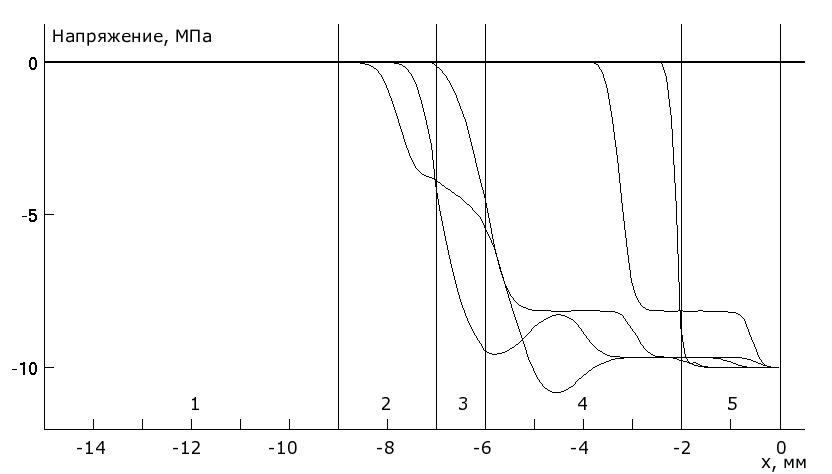
\includegraphics[width=0.8\textwidth]{png/cranium/multi-comp-model-1d.png}}
\caption{Многокомпонентная модель. 1 -- мозговое вещество, 2 -- ликвор, 3 -- внутренний слой компактной костной ткани, 4 -- слой губчатой костной ткани, 5 -- внешний слой компактной костной ткани.}
\label{pic:cranium_model1_1d}
\end{figure}

\begin{figure}[h]
\center{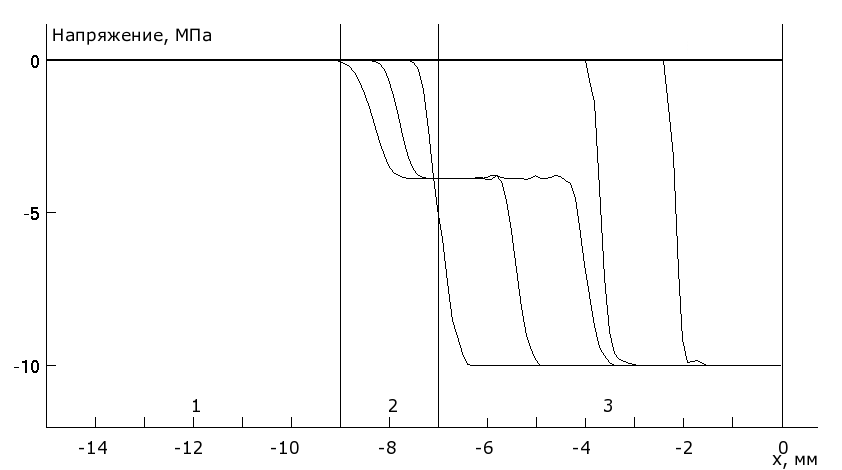
\includegraphics[width=0.8\textwidth]{png/cranium/single-comp-model-1d.png}}
\caption{Модель с однородным черепом из компактной костной ткани. 1 -- мозговое вещество, 2 -- ликвор, 3 -- череп из компактной костной ткани.}
\label{pic:cranium_model2_1d}
\end{figure}

Из графиков на рис. \ref{pic:cranium_model1_1d} и \ref{pic:cranium_model2_1d} видно, что волновые картины для разных моделей кардинально различаются. Большее количество контактных границ в многокомпонентной модели определяет существенно более сложную волновую картину.

В двумерной постановке моделировался удар шариком из жесткого пластика сантиметрового диаметра, налетающим со скоростью 3 м/с перпендикулярно стенке черепа. Принципиальная картина волновых процессов не зависит от скорости шарика, поэтому ее можно выбрать малой для удобства расчетов. 

На правой границе, соответствующей внешней стенке черепа, (рис. \ref{pic:cranium_calc_model}) ставилось условие свободной границы. На трех остальных границах также ставилось условие свободной границы, но при этом геометрия области выбиралась таким образом, чтобы за рассматриваемое время сильное возмущение не успело дойти до этих границ. Расчет различных слоев костной ткани черепа, внутричерепной жидкости и мозгового вещества производился сквозным образом.

На рис. \ref{pic:cranium_2d_simple_model} изображены изолинии напряжений в различные моменты времени, полученные с использованием упрощённой модели. Для многокомпонентной модели аналогичные картины приведены выше на рис. \ref{pic:cranium_2d}. Видно, что на начальной стадии, пока картина еще носит ярко выраженный волновой характер, распределение напряжений в случае использования разных моделей покровов мозга сильно отличается.

На относительно больших временах (в 10--15 раз больших, чем время прохождения волны через покровы мозга), когда волновые процессы выражены уже относительно слабо и возмущения в заметной степени проникают в мозг, основную роль начинает играть различие механических свойств черепа и мозга. Так как оно на порядки больше, чем различие свойств компонент черепа между собой, то на этой стадии внутреннее строение черепа мало влияет на итоговую картину. Результаты расчетов по разным моделям на этом этапе отличаются между собой незначительно.


\begin{figure}[h]
\centering
\begin{subfigure}[b]{0.13\textwidth}
\centering

\includegraphics[width=\textwidth]{png/cranium/2d-sxx-single-comp-01.png}
\caption{ }
\end{subfigure}
\begin{subfigure}[b]{0.13\textwidth}
\centering

\includegraphics[width=\textwidth]{png/cranium/2d-sxx-single-comp-02.png}
\caption{ }
\end{subfigure}
\begin{subfigure}[b]{0.13\textwidth}
\centering

\includegraphics[width=\textwidth]{png/cranium/2d-sxy-single-comp-01.png}
\caption{ }
\end{subfigure}
\begin{subfigure}[b]{0.13\textwidth}
\centering

\includegraphics[width=\textwidth]{png/cranium/2d-sxy-single-comp-02.png}
\caption{ }
\end{subfigure}
\begin{subfigure}[b]{0.13\textwidth}
\centering

\includegraphics[width=\textwidth]{png/cranium/2d-syy-single-comp-01.png}
\caption{ }
\end{subfigure}
\begin{subfigure}[b]{0.13\textwidth}
\centering

\includegraphics[width=\textwidth]{png/cranium/2d-syy-single-comp-02.png}
\caption{ }
\end{subfigure}
\caption{Модель с однородным черепом из компактной костной ткани.  Изолинии напряжений. а -- $\sigma_{xx}$ при t = 7.5 мкс., б -- $\sigma_{xx}$ при t = 12.5 мкс., в -- $\sigma_{xy}$ при t = 7.5 мкс., г -- $\sigma_{xy}$ при t = 12.5 мкс., д -- $\sigma_{yy}$ при t = 7.5 мкс., е -- $\sigma_{yy}$ при t = 12.5 мкс. Ось x направлена вправо, ось y -- вверх. Шарик налетает справа.}
\label{pic:cranium_2d_simple_model}
\end{figure}

\clearpage
\newpage

\subsubsection*{Моделирование системы череп-мозг}

Для моделирования системы череп-мозг использовалось несколько механико-математических моделей головы человека. Простейшей из них является двухкомпонентная модель (рис. \ref{pic:cranium_2d_problem}а), в которой ткани кости и мозга описываются однородными изотропными материалами, имеющими усредненные механические свойства. Более сложные модели учитывают наличие желудочка (рис. \ref{pic:cranium_2d_problem}б) и мембраны твердой оболочки (рис. \ref{pic:cranium_2d_problem}в). Соответствующие расчетные сетки приведены на рис. \ref{pic:cranium_2d_mesh}.

Реологические свойства биоматериалов приведены в таблице \ref{tbl:cranium_elastic_parameters}. Поведение костного материала моделировалась как изотропная линейноупругая сплошная среда со средними свойствами пластинчатой и губчатой кости.

Моделирование взаимодействия между черепом и мозгом является сложной задачей ввиду того, что в действительности мозг имеет большое количество различных по механическим свойствам оболочек, складчатых структур, врастающих друг в друга, с полостями, заполненными жидкостью (ликвором). В данной работе применялся метод явного выделения контактного разрыва с контактными условиями скольжения.

Внешняя нагрузка задавалась как соударение системы череп-мозг с абсолютно жесткой неподвижной преградой с заданной начальной скоростью (1--3 м/с).

\begin{figure}[h]
\centering
\begin{subfigure}[b]{0.3\textwidth}
\centering
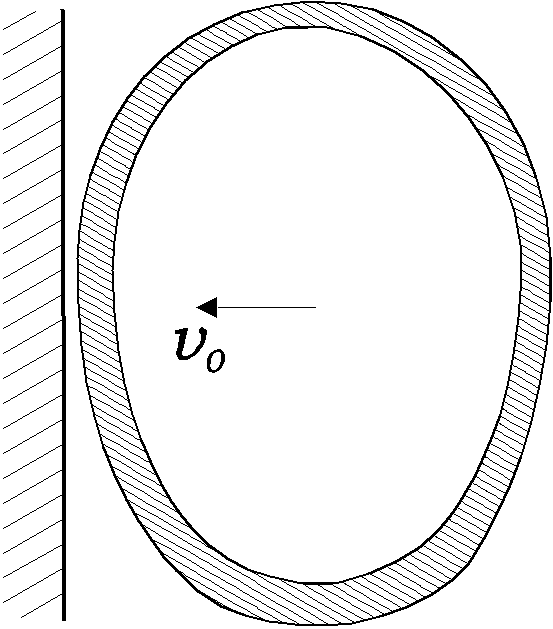
\includegraphics[width=\textwidth]{png/cranium/2d-problem-1.png}
\caption{Двухкомпонентная модель}
\end{subfigure}
\begin{subfigure}[b]{0.3\textwidth}
\centering
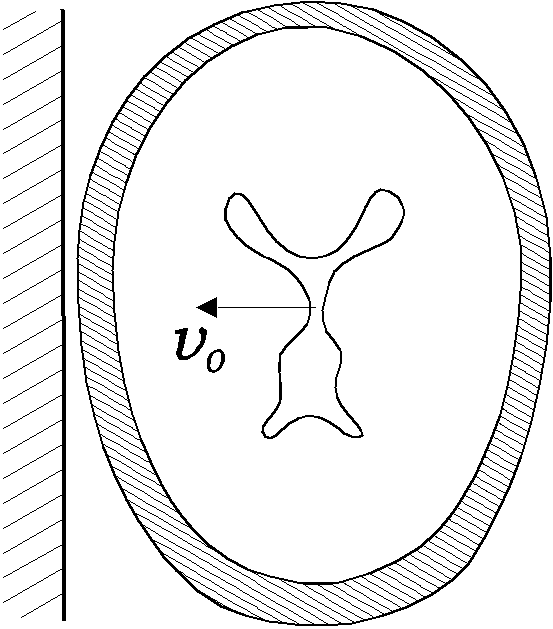
\includegraphics[width=\textwidth]{png/cranium/2d-problem-2.png}
\caption{Модель с желудочками}
\end{subfigure}
\begin{subfigure}[b]{0.3\textwidth}
\centering
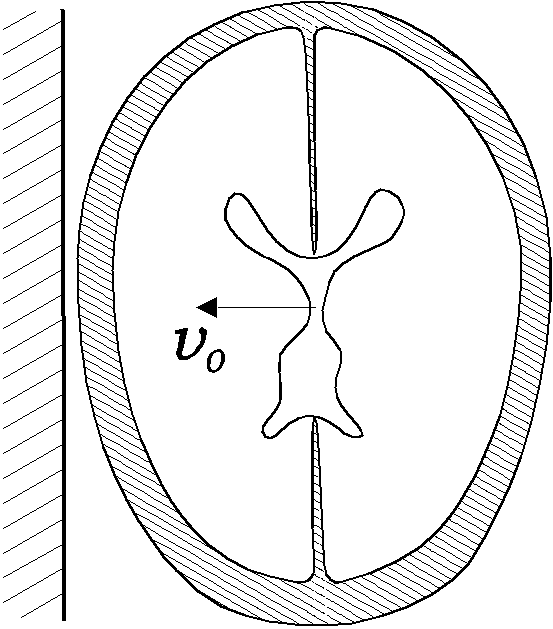
\includegraphics[width=\textwidth]{png/cranium/2d-problem-3.png}
\caption{Модель с желудочками и мембраной}
\end{subfigure}
\caption{Использованные модели головы человека.}
\label{pic:cranium_2d_problem}
\end{figure}



\begin{figure}[h]
\centering
\begin{subfigure}[b]{0.3\textwidth}
\centering
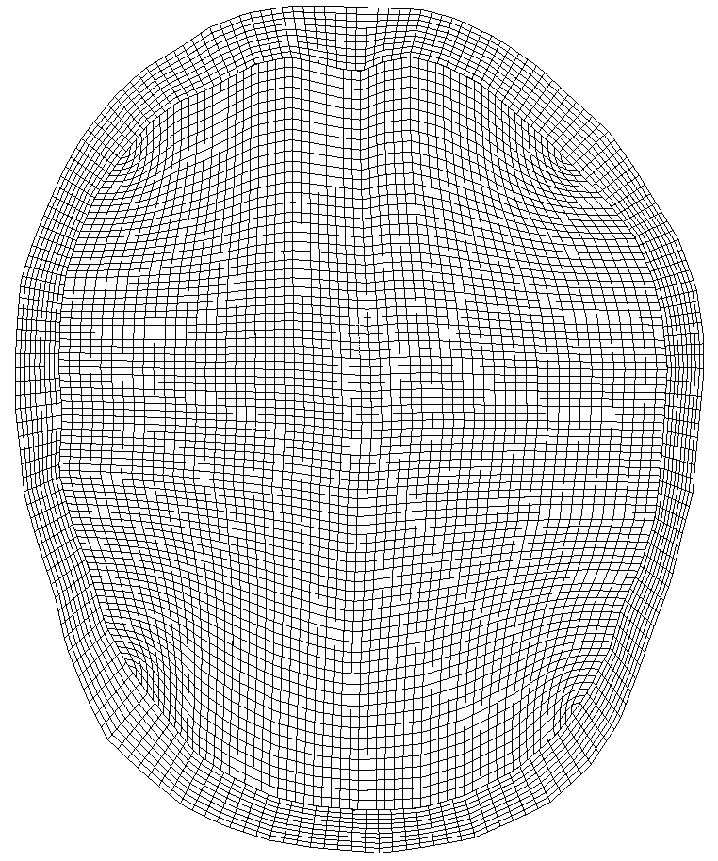
\includegraphics[width=\textwidth]{png/cranium/2d-problem-mesh-1.png}
\caption{Двухкомпонентная модель}
\end{subfigure}
\begin{subfigure}[b]{0.3\textwidth}
\centering
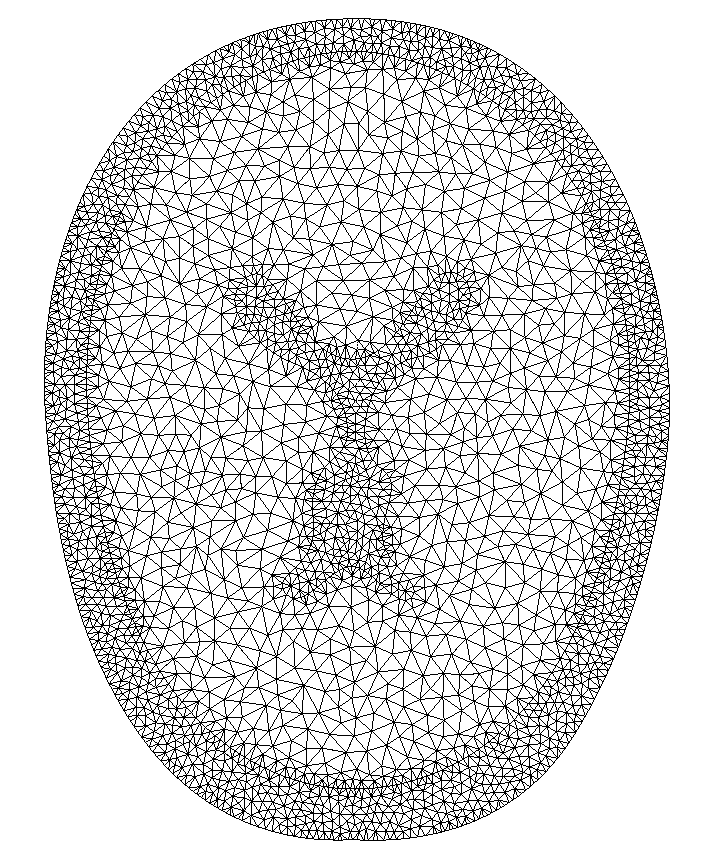
\includegraphics[width=\textwidth]{png/cranium/2d-problem-mesh-2.png}
\caption{Модель с желудочками}
\end{subfigure}
\begin{subfigure}[b]{0.3\textwidth}
\centering
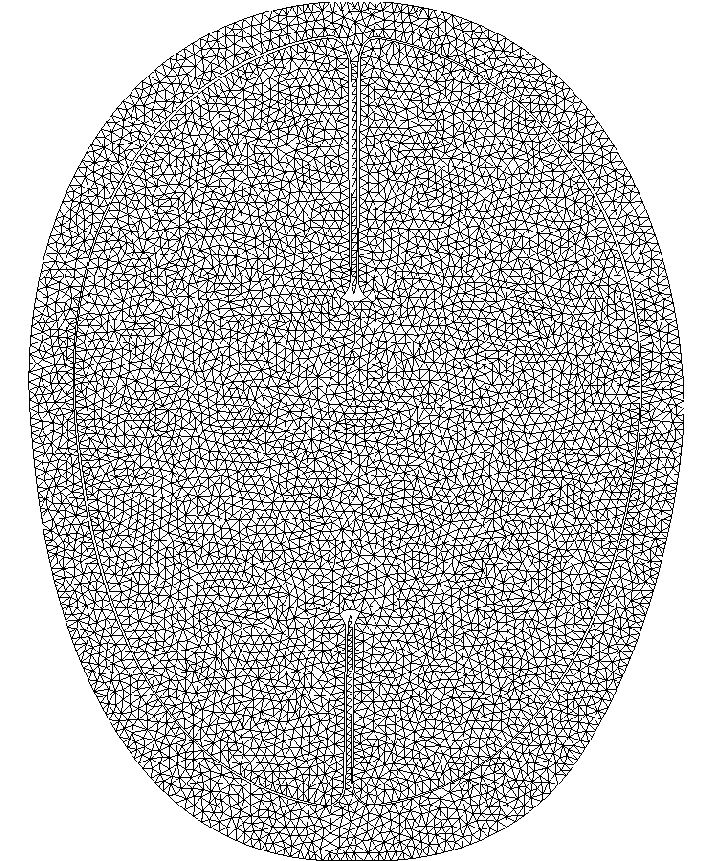
\includegraphics[width=\textwidth]{png/cranium/2d-problem-mesh-3.png}
\caption{Модель с желудочками и мембраной}
\end{subfigure}
\caption{Расчетные сетки для моделей головы человека.}
\label{pic:cranium_2d_mesh}
\end{figure}

На рис. \ref{pic:cranium_2d_res_1} приведены интегральные характеристики механического воздействия на мозг при боковом ударе, полученные с помощью двухкомпонентной модели с условием свободного скольжения на границе череп-мозг. Наиболее опасными представляются концентрации максимальных растягивающих (рис. \ref{pic:cranium_2d_res_1}б) и сдвиговых напряжений (рис. \ref{pic:cranium_2d_res_1}в). В частности, упомянутое выше явление противоудара продемонстрировано на рис. \ref{pic:cranium_2d_res_1}б -- наиболее опасные повреждения мозгового вещества локализуются в области положительных напряжений.

\begin{figure}[h]
\centering
\begin{subfigure}[b]{0.3\textwidth}
\centering
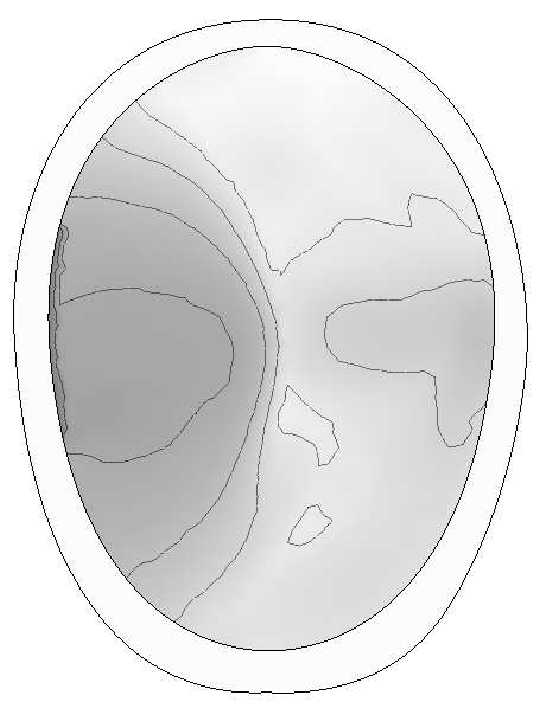
\includegraphics[width=\textwidth]{png/cranium/2d-problem-res-1.png}
\caption{Максимальное напряжение сжатия}
\end{subfigure}
\begin{subfigure}[b]{0.3\textwidth}
\centering
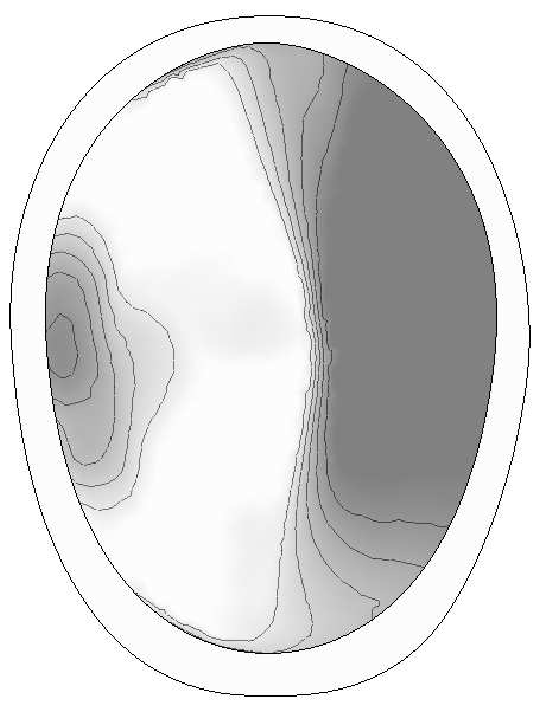
\includegraphics[width=\textwidth]{png/cranium/2d-problem-res-2.png}
\caption{Максимальное напряжение растяжения}
\end{subfigure}
\begin{subfigure}[b]{0.3\textwidth}
\centering
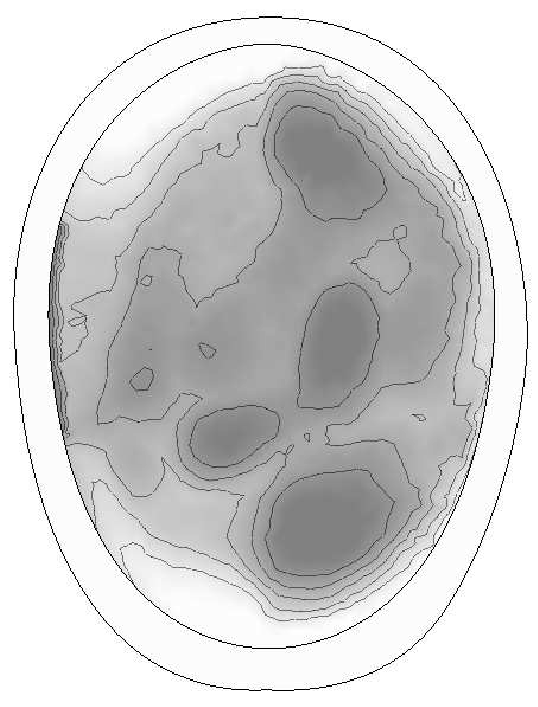
\includegraphics[width=\textwidth]{png/cranium/2d-problem-res-3.png}
\caption{Максимальное сдвиговое напряжение}
\end{subfigure}
\caption{Результаты расчета двухкомпонентной модели.}
\label{pic:cranium_2d_res_1}
\end{figure}

На рис. \ref{pic:cranium_2d_res_2} приведены распределения сдвиговых напряжений при ударе снизу, полученные с помощью разных моделей. Использование условия полного слипания на границе череп-мозг приводит к концентрации сдвиговых напряжений вдоль контактной границы на боковых поверхностях, в то время как скользящий контакт полностью их снимает. Учет наличия желудочков оказывает слабое влияние на распределение областей максимального сжатия и растяжения, но существенно влияет на распределение сдвиговых нагрузок. Наличие мембраны является более существенным для локализации областей сжатия-растяжения при боковых ударах.

\begin{figure}[h]
\centering
\begin{subfigure}[b]{0.3\textwidth}
\centering
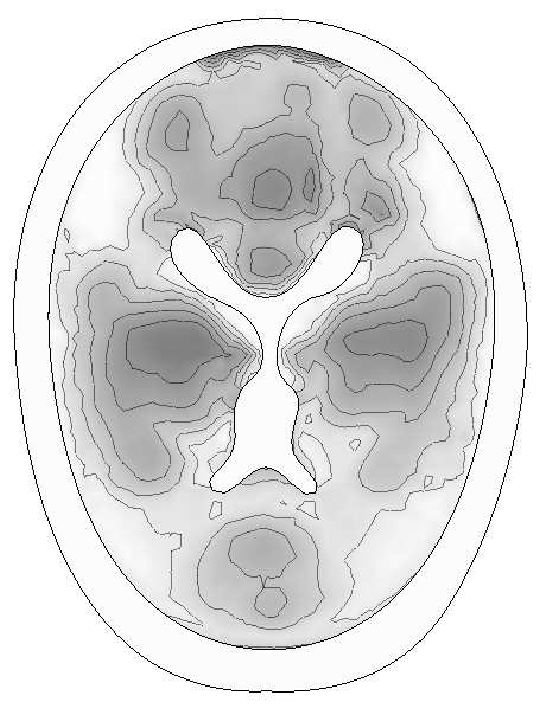
\includegraphics[width=\textwidth]{png/cranium/2d-problem-res-4.png}
\caption{Полное слипание на контактной границе}
\end{subfigure}
\begin{subfigure}[b]{0.3\textwidth}
\centering
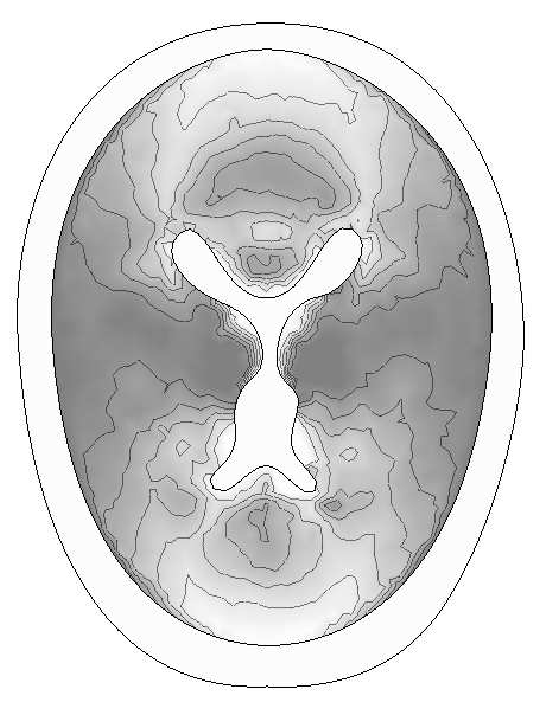
\includegraphics[width=\textwidth]{png/cranium/2d-problem-res-5.png}
\caption{Свободное скольжение на контактной границе}
\end{subfigure}
\begin{subfigure}[b]{0.3\textwidth}
\centering
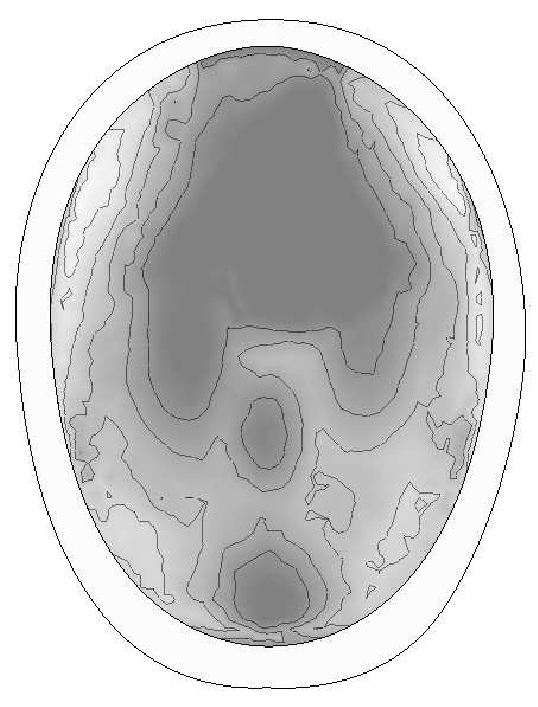
\includegraphics[width=\textwidth]{png/cranium/2d-problem-res-6.png}
\caption{Двухкомпонентная модель, слипание}
\end{subfigure}
\caption{Распределение сдвиговых напряжений для разных моделей.}
\label{pic:cranium_2d_res_2}
\end{figure}


\clearpage
\newpage


\subsection{Задача о динамическом нагружении коленного сустава}

Колени -- очень уязвимая часть организма человека. Отдельное внимание при рассмотрении повреждений коленного сустава следует уделить мениску. Заметное изнашивание или тем более разрыв мениска делает работу коленного сустава практически невозможной. Кроме того, мениск плохо снабжается кровью, поэтому сам по себе он не заживает и не восстанавливается. Мениск выполняет не только функцию амортизатора, но и заполняет пространство между костями.

Колено представляет собой сложную механическую структуру (рис. \ref{pic:knee_scheme}), поэтому процессы повреждения, протекающие в нём, тоже сложны. С помощью численного моделирования можно воспроизвести травмы, характер их развития. Другое не менее важное применение моделирования в данной задаче -- численное воспроизведение хирургической операции, например пересадки мениска. 

\begin{figure}[h]
\center{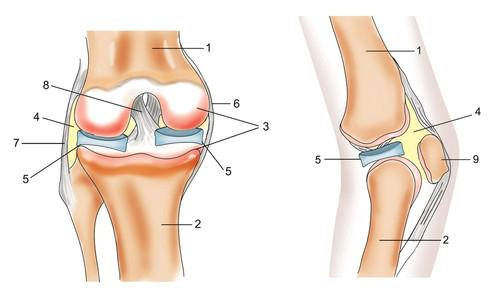
\includegraphics[width=\textwidth]{png/cranium/knee-scheme.png}}
\caption{Строение коленного сустава: 1 - бедренная кость, 2 - большая берцовая кость, 3 - хрящи, 4 - полость с жидкостью, 5 - внутренний и внешний мениски, 6 - внешняя связка, 7 - внутренняя связка, 8 - крестообразная связка, 9 - надколенник.}
\label{pic:knee_scheme}
\end{figure}

\clearpage
\newpage

Наиболее распространенные травмы коленного сустава при относительно слабых воздействиях -- повреждения мягких тканей, к которым относятся гематомы, растяжения и разрыв связок и мениска, а также вывихи коленной чашечки и коленного сустава. Эти травмы являются следствиями прямого воздействия на колено, скручивания ноги или чрезмерного сгибания.

В рамках данной работы рассматривается модель согнутого коленного сустава (рис. \ref{pic:knee_model}а), включающая берцовую кость, бедренную кость, коленную чашечку и мениск. Соответствующая расчетная сетка приведена на рис. \ref{pic:knee_model}б. Значения параметров биологических сред приведены в таблице \ref{tbl:knee_elastic_parameters}.


\begin{figure}[h]
\centering
\begin{subfigure}[b]{0.4\textwidth}
\centering
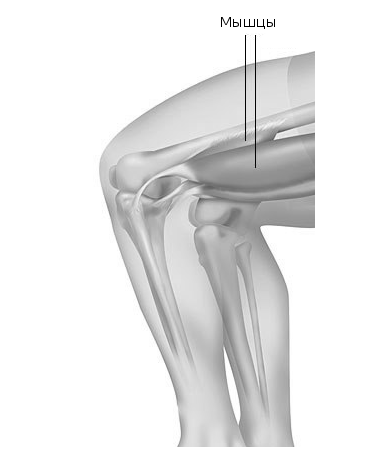
\includegraphics[width=\textwidth]{png/cranium/knee-strike.png}
\caption{Схема.}
\end{subfigure}
\begin{subfigure}[b]{0.4\textwidth}
\centering
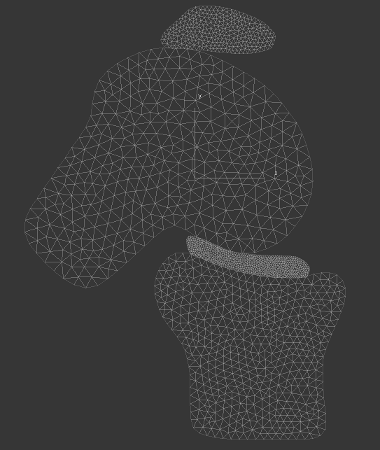
\includegraphics[width=\textwidth]{png/cranium/knee-mesh.png}
\caption{Расчетная сетка.}
\end{subfigure}
\caption{Согнутый коленный сустав.}
\label{pic:knee_model}
\end{figure}

\begin{table}[h]
\centering
\caption{Механические характеристики в задаче о коленном суставе}
\begin{tabular}{|c|c|c|c|}
\hline
Компонент & $\rho$, кг/м$^{3}$ & $\lambda$, ГПа & $\mu$, ГПа  \\
\hline
Костная ткань & 1.60 & 2100 & 2700 \\
Мягкие ткани мениска & 1.10 & 100 & 70 \\
\hline
\end{tabular}
\label{tbl:knee_elastic_parameters}
\end{table}

\clearpage
\newpage

В первом расчете скорость соударения составляла 3 м/с, направление удара составляло 45 градусов с горизонталью. Распределение напряжений показано на рис. \ref{pic:knee_res_1}. При этой скорости удара напряжения, возникающие в кости, значительно меньше предела прочности костной ткани. Однако, напряжения сжатия и растяжения в мениске достигают 1-2 МПа, что согласно \cite{dlima} может вызывать повреждения менисковой ткани. Сдвиговые напряжения не превышают 1 МПа, что не представляет опасности ни для костной, ни для менисковой тканей.

\begin{figure}[H]
\center{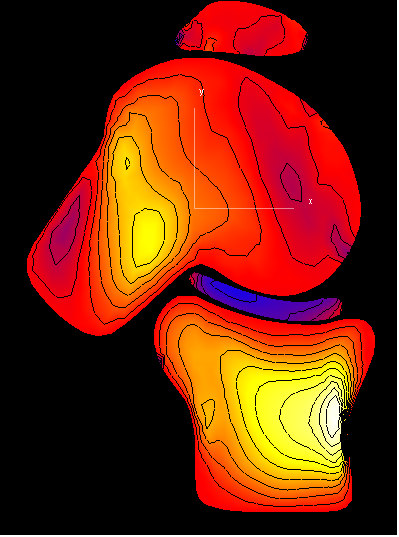
\includegraphics[width=0.6\textwidth]{png/cranium/knee-res-1.png}}
\caption{Распределение напряжений сжатия / растяжения. Скорость удара 3 м/с.}
\label{pic:knee_res_1}
\end{figure}

Во втором расчете скорость составляла 9 м/с. Распределение напряжений показано на рис. \ref{pic:knee_res_2}.

\clearpage
\newpage

\begin{figure}[h]
\centering
\begin{subfigure}[b]{0.6\textwidth}
\centering
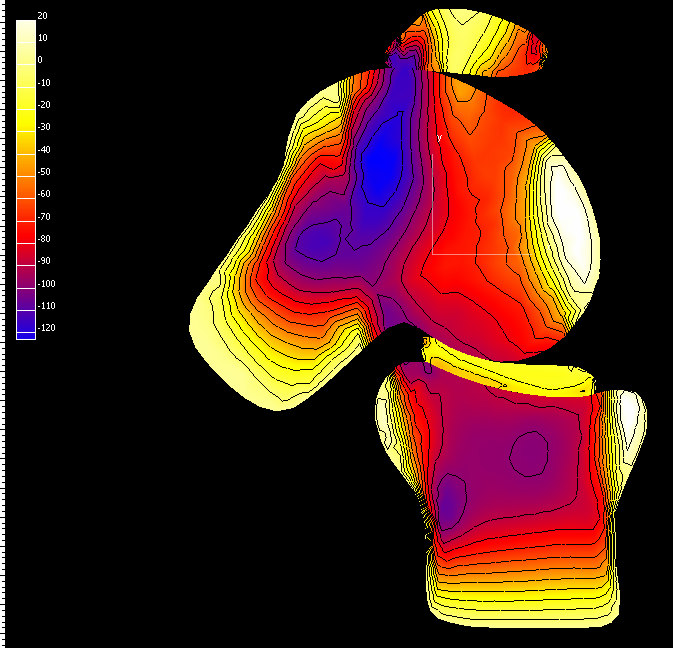
\includegraphics[width=\textwidth]{png/cranium/knee-res-2.png}
\caption{Начальный момент удара}
\end{subfigure}
\begin{subfigure}[b]{0.6\textwidth}
\centering
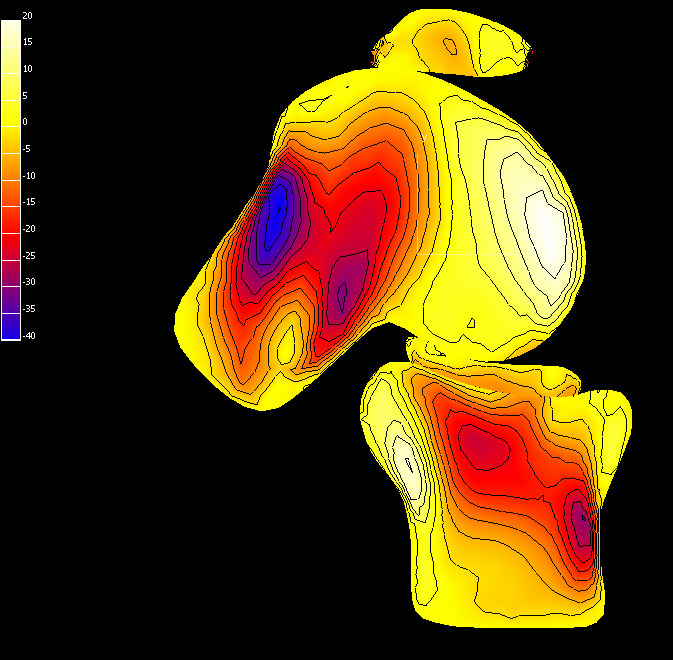
\includegraphics[width=\textwidth]{png/cranium/knee-res-3.png}
\caption{Завершающая стадия удара}
\end{subfigure}
\caption{Распределение напряжений сжатия / растяжения. Скорость удара 9 м/с.}
\label{pic:knee_res_2}
\end{figure}

\clearpage
\newpage

При такой скорости в кости возникают напряжения сжатия до величин порядка сотни МПа, что не превышает предела прочности костной ткани. Однако, напряжение растяжения костная ткань выдерживает значительно хуже, при нагрузке растяжения порядка 50-70 МПа уже могут возникать переломы \cite{begun}. Области максимальных растяжений на рисунке \ref{pic:knee_res_2} показаны белым, в этих областях возможны переломы.

Одной из характерных травм при ударе по коленному суставу является перелом мыщелка большеберцовой кости. Механизм формирования данной травмы схематически изображен на рис. \ref{pic:knee_crack_scheme}. Видно, что области повреждений с хорошей точностью совпадают с зонами максимальных растягивающих напряжений, полученными в расчете (см. рис. \ref{pic:knee_res_2}).

\begin{figure}[h]
\center{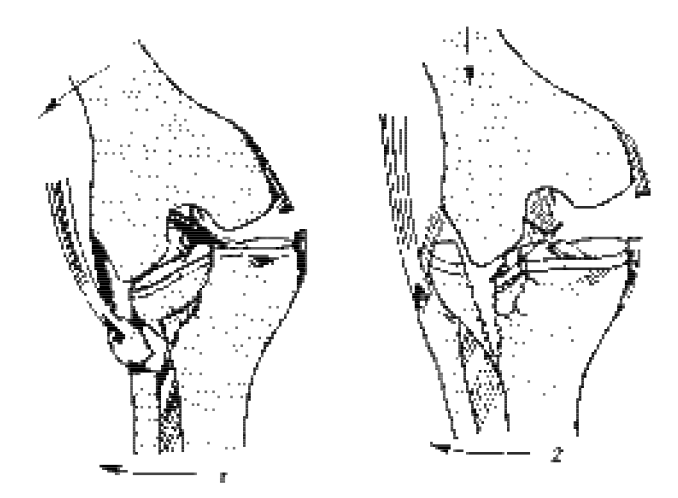
\includegraphics[width=0.8\textwidth]{png/cranium/knee-crack-scheme.png}}
\caption{Механизм повреждения при двух типах перелома наружного мыщелка большеберцовой кости.}
\label{pic:knee_crack_scheme}
\end{figure}


\clearpage
\newpage


\subsection{Задача об ударе по грудной клетке в защитной конструкции}

В медицинской практике известны случаи внезапной остановки сердца молодых спортсменов в результате низкоинтенсивного непроникающего воздействия тупого предмета на прекардиальную область (в основном не очень сильные удары в грудь хоккейной шайбой или бейсбольным мячом). Патогенез этих смертей неясен. Вероятно, удар в грудь попадает в уязвимый период сердечного цикла и вызывает желудочковую тахикардию или фибрилляцию желудочков. Подобные травмы приводили к летальному исходу даже в тех случаях, когда на спортсменах присутствовала защитная амуниция. Следовательно, существующие на сегодняшний день средства защиты неэффективны при определенных типах воздействия. Соответственно, требуется исследование возможных факторов остановки сердца при таких воздействиях, что позволит разработать новые типы протекторов грудной клетки.

\begin{figure}[h]
\center{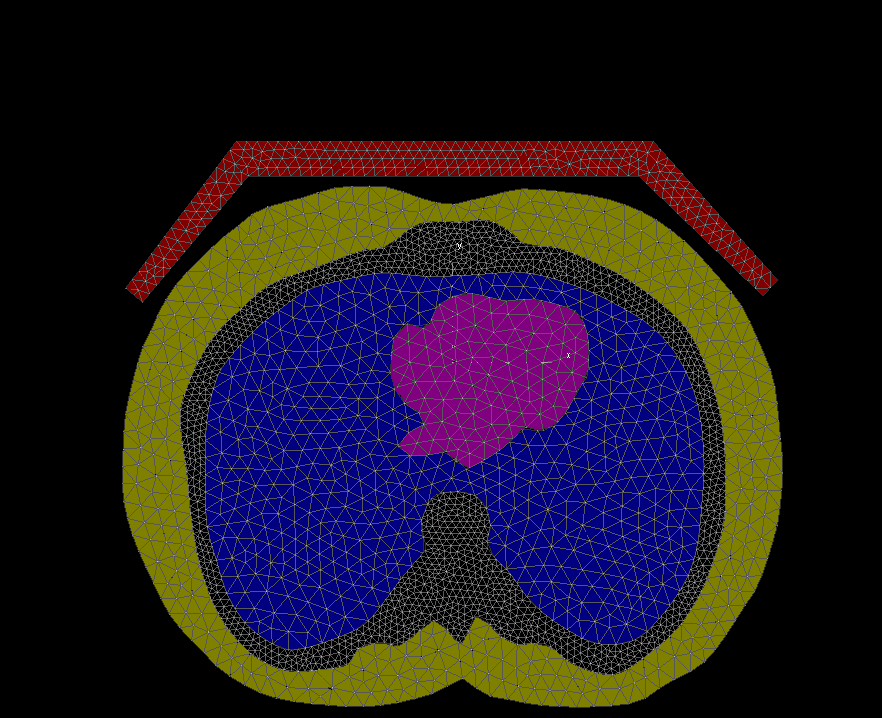
\includegraphics[width=0.8\textwidth]{png/cranium/chest-scheme.png}}
\caption{Модель грудной клетки: мышечная ткань, костная ткань ребер, мягкие ткани внутренних органов, сердечная мышца.}
\label{pic:chest_scheme}
\end{figure}

В рамках данной работы рассматривается модель грудной клетки, включающая сердце, слой мягких тканей внутренних органов, рёбра и слой мягких тканей мышц (рис. \ref{pic:chest_scheme}). Параметры костной ткани и мягких тканей приведены в таблице \ref{tbl:chest_elastic_parameters}. Контактное условие на границах между тканями грудной клетки -- полное слипание. Контактное условие между тканями грудной клетки и защитной амуницией -- свободное скольжение. Рассматривается удар под углом 45 градусов со скоростью 4 м/с. 

\begin{table}[h]
\centering
\caption{Механические характеристики в задаче о грудной клетке}
\begin{tabular}{|c|c|c|c|}
\hline
Компонент & $\rho$, кг/м$^{3}$ & $\lambda$, ГПа & $\mu$, ГПа  \\
\hline
Костная ткань & 1.60 & 2100 & 2700 \\
Мягкие ткани & 1.10 & 100 & 70 \\
\hline
\end{tabular}
\label{tbl:chest_elastic_parameters}
\end{table}


\begin{figure}[h]
\centering
\begin{subfigure}[b]{0.9\textwidth}
\centering
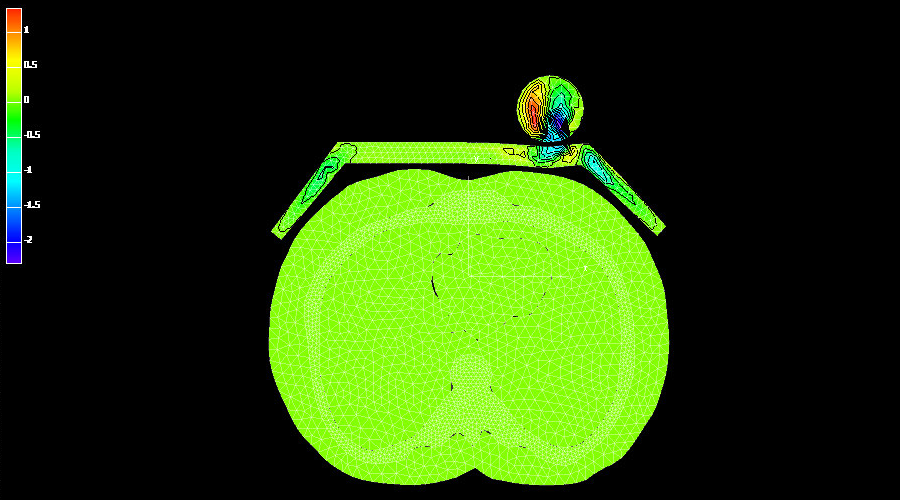
\includegraphics[width=\textwidth]{png/cranium/chest-res-01.png}
\end{subfigure}
\caption{Прохождение волны через защитную конструкцию.}
\end{figure}


\begin{figure}[h]
\centering
\begin{subfigure}[b]{0.9\textwidth}
\centering
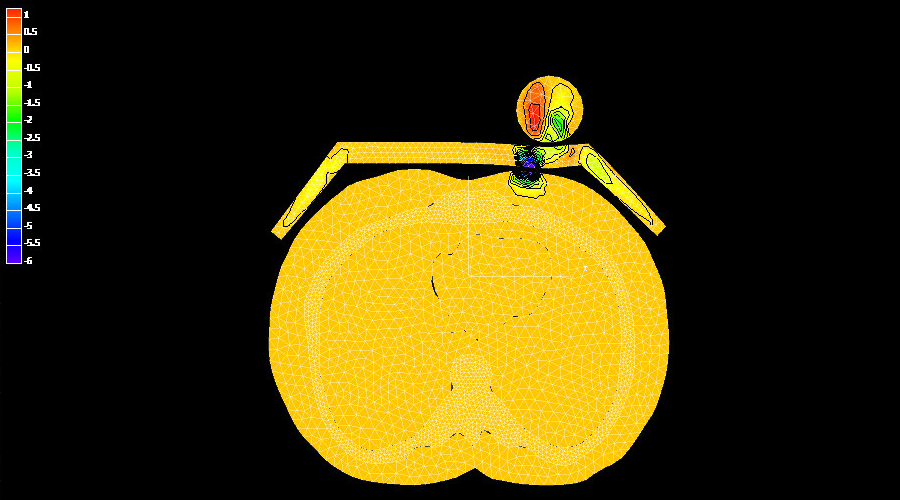
\includegraphics[width=\textwidth]{png/cranium/chest-res-02.png}
\caption{ }
\end{subfigure}
\begin{subfigure}[b]{0.9\textwidth}
\centering
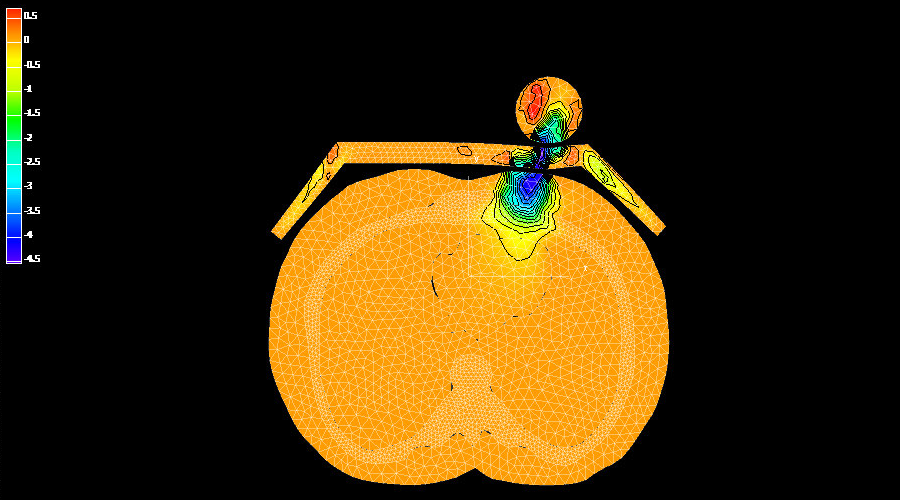
\includegraphics[width=\textwidth]{png/cranium/chest-res-03.png}
\caption{ }
\end{subfigure}
\caption{Проникновение возмущения в мягкие ткани.}
\end{figure}


\begin{figure}[h]
\centering
\begin{subfigure}[b]{0.9\textwidth}
\centering
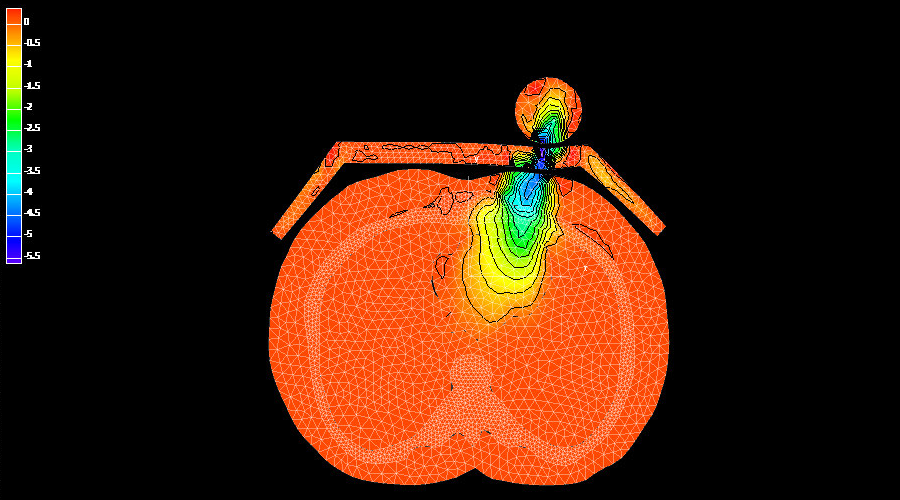
\includegraphics[width=\textwidth]{png/cranium/chest-res-04.png}
\caption{ }
\end{subfigure}
\begin{subfigure}[b]{0.9\textwidth}
\centering
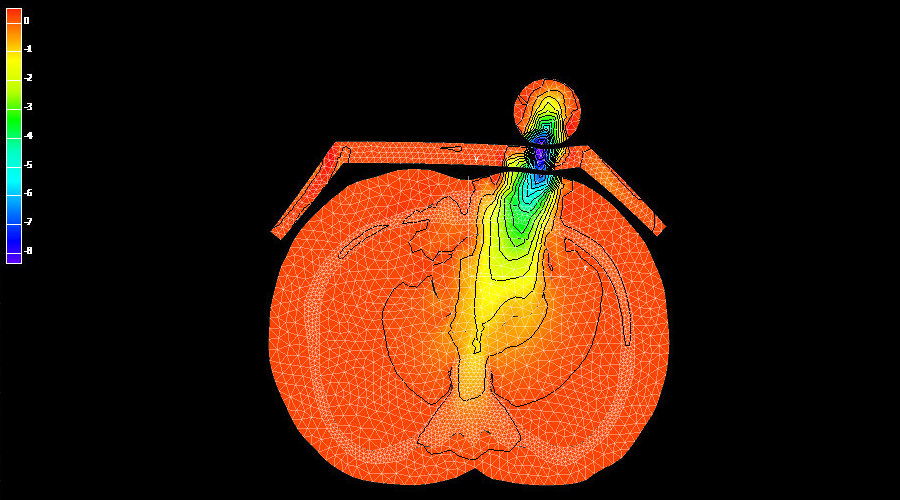
\includegraphics[width=\textwidth]{png/cranium/chest-res-05.png}
\caption{ }
\end{subfigure}
\caption{Прохождение возмущения через костную ткань в область сердечной мышцы.}
\end{figure}

\begin{figure}[h]
\centering
\begin{subfigure}[b]{0.9\textwidth}
\centering
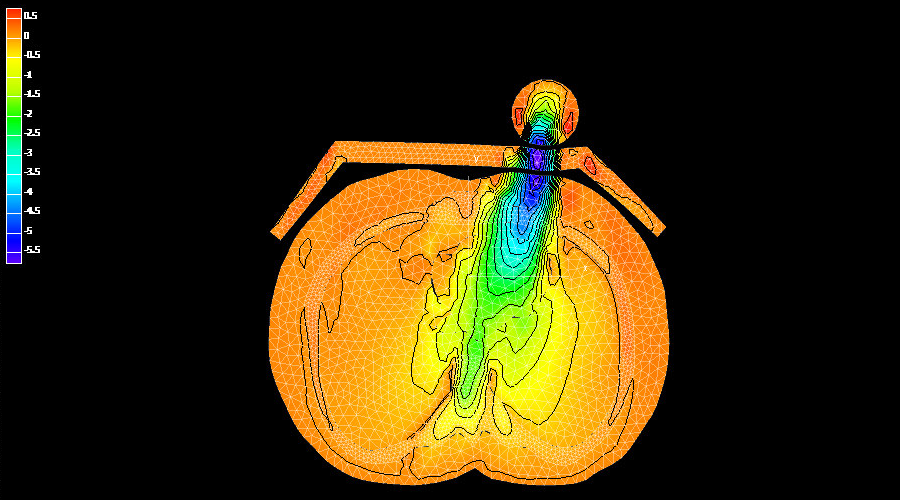
\includegraphics[width=\textwidth]{png/cranium/chest-res-06.png}
\caption{Момент максимальной концентрации напряжений в области сердечной мышцы}
\end{subfigure}
\begin{subfigure}[b]{0.9\textwidth}
\centering
\includegraphics[width=\textwidth]{png/cranium/chest-res-07.png}
\caption{Завершающая стадия соударения, отскок ударника}
\end{subfigure}
\caption{Поздние стадии соударения}
\end{figure}

